\documentclass[12pt,fontset=windows]{ctexart}

\usepackage{geometry} % 绘制公式
\usepackage{graphicx}
\usepackage{mathrsfs}%使用花体字母
\usepackage{amsfonts}%使用双线体
\usepackage{mathtools}%使用coloneqq符号
\usepackage{amsmath}
\usepackage{xcolor} % 适用颜色框
\usepackage{tcolorbox}
\usepackage{titling} % 用于调整标题的垂直间距
% \usepackage{hyperref}%公式超链接
\usepackage[colorlinks,
linkcolor=red,
anchorcolor=blue,
citecolor=green
]{hyperref}
\usepackage{listings}
\usepackage{array}
\usepackage{booktabs}
\usepackage{algorithm}  
\usepackage{algpseudocode}  
\usepackage{amsmath}  
\usepackage{cases}

\newcommand{\CASE}[1]{\textbf{case} #1\textbf{: } }
\renewcommand{\algorithmicrequire}{\textbf{Input:}}  % Use Input in the format of Algorithm  
\renewcommand{\algorithmicensure}{\textbf{Output:}} % Use Output in the format of Algorithm 


\geometry{
	a4paper, % 使用A4纸张
	left=20mm, % 左侧页边距为20毫米
	right=20mm, % 右侧页边距为20毫米
	top=25mm, % 顶部页边距为25毫米
	bottom=25mm % 底部页边距为25毫米
}

% 自定义环境“!”代表透明度可调节
\tcbset{
	blue/.style={
		colback=blue!10!white,
		colframe=black,
		boxrule=1pt,
		arc=0mm,
		auto outer arc,
		left=1mm,
		right=1mm,
		top=1mm,
		bottom=1mm
	}
}
\tcbset{
	green/.style={
		colback=green!10!white,
		colframe=black,
		boxrule=1pt,
		arc=0mm,
		auto outer arc,
		left=1mm,
		right=1mm,
		top=1mm,
		bottom=1mm
	}
}
\tcbset{
	red/.style={
		colback=red!5!white,
		colframe=black,
		boxrule=1pt,
		arc=0mm,
		auto outer arc,
		left=1mm,
		right=1mm,
		top=1mm,
		bottom=1mm
	}
}
\tcbset{
	cyan/.style={
		colback=cyan!40!white,
		colframe=black,
		boxrule=1pt,
		arc=0mm,
		auto outer arc,
		left=1mm,
		right=1mm,
		top=1mm,
		bottom=1mm
	}
}

\lstset{
 columns=fixed,       
 numbers=left,                                        % 在左侧显示行号
 numberstyle=\tiny\color{gray},                       % 设定行号格式
 frame=none,                                          % 不显示背景边框
 backgroundcolor=\color[RGB]{245,245,244},            % 设定背景颜色
 keywordstyle=\color[RGB]{40,40,255},                 % 设定关键字颜色
 numberstyle=\footnotesize\color{darkgray},           
 commentstyle=\it\color[RGB]{0,96,96},                % 设置代码注释的格式
 stringstyle=\rmfamily\slshape\color[RGB]{128,0,0},   % 设置字符串格式
 showstringspaces=false,                              % 不显示字符串中的空格
 language=c++,                                        % 设置语言
}


% 调整标题的垂直间距
\setlength{\droptitle}{-60pt}
\pretitle{\begin{center}\LARGE\bfseries\vskip -20pt}
\posttitle{\par\vskip -10pt\rule{\textwidth}{0.4pt}\vskip -10pt\end{center}}
\predate{\begin{center}\large\vskip -10pt}
\postdate{\par\vskip -10pt\rule{\textwidth}{0.4pt}\vskip -20pt\end{center}}

\title{MINCO轨迹类航点硬约束处理}

\author{郑一品}
\date{2024年10月9日} % 可以将日期留空,或者填写你希望显示的日期


\begin{document}
    
\maketitle
\section{2024年10月9日}
\begin{tcolorbox}[cyan]
    \begin{description}
        \item[\large \textbf{任务}]
        \item[1、] GCOPTER源代码
        \item[2、] Geometrically Constrained Trajectory Optimization for Multicopters 论文研究
        \item[3、] Polynomial-based Online Planning for Autonomous Drone Racing in Dynamic Environments对比\textbf{2}的提升
    \end{description}
\end{tcolorbox}
\subsection{Geometrically Constrained Trajectory Optimization for Multicopters(T-RO2022)}
\subsubsection{凸多面体几何约束的处理}
对于凸多面体,其表示形式有以下两种;


(1)\textbf{$\mathcal{V}$-多面体}: $\mathbb{R} ^d$中的有限点集$X=\{x^{1},\ldots,x^{n}\}$所构成的凸包,
\begin{equation}
    P^\mathcal{V}=\operatorname{conv}(X) := \{\sum_{i=1}^n\lambda_ix^i \Big| \lambda_1,\ldots,\lambda_n\geq0,
     \sum_{i=1}^n\lambda_i=1\Big\}.
\end{equation}


(2)\textbf{$\mathcal{H}$-多面体}:有限线性不等式方程组的解集,
\begin{equation}
    P^\mathcal{H}=P(A,b) := \big\{x\in\mathbb{R}^d\mid a_i^Tx\leq b_i\text{ for }1\leq i\leq m\big\}.
\end{equation}
其中,$A\in\mathbb{R}^{m \times b} $是一个以$a_i^T$为行的实矩阵,$b\in\mathbb{R}^b $是一个以$b_i$为项的实向量,即
\begin{equation}\label{polytope}
    P^\mathcal{H}= \{x\in \mathbb{R}^n| \mathbf{A}x\preceq b\}  .
\end{equation}
\begin{tcolorbox}[green]
    \textbf{欧式空间到球体的映射:}考虑m维空间里以$o$为中心、$r$为半径的低维球约束,有如下形式:
    \begin{equation}
        \mathcal{P}^{\mathcal{B}}=\left\{x\in\mathbb{R}^n\mid\left\|x-o\right\|_2\leq r\right\}.
    \end{equation}
    利用光滑的满射将$\mathbb{R}^n$映射到$\mathcal{P}^{\mathcal{B}}$,
    便可以在$\mathbb{R}^n$的代理变量上进行优化隐式地满足$\mathcal{P}^{\mathcal{B}}$的约束。
\end{tcolorbox}
\begin{tcolorbox}[red]
    \textbf{映射1: 欧氏空间$\mathbb{R}^n$ $\rightarrow $ 球体}
    \begin{equation}\label{sqheretorn}
        x=o+\frac{2r\xi }{\xi^\mathrm{T}\xi+1}\in\mathcal{P}^\mathcal{B}, \forall \xi\in\mathbb{R}^n.
    \end{equation}
    其中,引入一个代理变量$\xi$,以$\xi$指代\textbf{q}的无约束代理变量。通过计算\eqref{sqheretorn}的Jacobian即可得到梯度
    \begin{equation}
        \frac{\partial J}{\partial\xi_i}=\frac{2r_ig_i}{\xi_i^\mathrm{T}\xi_i+1}-\frac{4r_i(\xi_i^\mathrm{T}g_i)\xi_i}{(\xi_i^\mathrm{T}\xi_i+1)^2}.
    \end{equation}
    其中,$g_i\text{ 代表 }\partial J/\partial\mathbf{q}\text{ 中的第 }i\text{ 个元素 }\partial J/\partial q_i$。
\end{tcolorbox}

\begin{tcolorbox}[green]
    \textbf{球体到凸多面体的映射:}考虑凸多面体$\mathcal{P} ^\mathcal{H}$,采用多面体的$\mathcal{V}$-表示,
    其顶点数目为$\hat{n} +1$,分别为$(v_0,v_1,\cdots ,v_{\hat{n}})$,
    其在重心坐标下等价于一个标准的$\hat{n}$-单纯形$\mathcal{P} ^\mathcal{H}_\omega $,
    在平方变量代换下,$\mathcal{P} ^\mathcal{H}_\omega $等价于一个$\hat{n}$维球。
\end{tcolorbox}
\begin{tcolorbox}[red]
    \textbf{映射2: 单纯形 $\rightarrow $ 凸多面体}
    \begin{equation}\label{1}
        q = v_0 + \mathbf{\hat{V}}\mathbf{\omega}
    \end{equation}
    其中,$q\in\mathcal{P}^\mathcal{H}$,$\mathbf{\hat{V}}= (\hat{v_1},\hat{v_2},\cdots, \hat{v_{\widehat{n}}})$,
    $\hat{v_i}= v_i-v_0$,$\mathbf{\omega}=(\omega_1,\cdots,\omega_{\widehat{n}})^T$。由如下单纯形映射到凸多面体\eqref{polytope}:
    \begin{equation}\label{simplex}
        \mathcal{P}_w^\mathcal{H}=\left\{w\in\mathbb{R}^{\hat{n}} \bigg| w\succeq0, \|w\|_1\leq1\right\}.
    \end{equation}
\end{tcolorbox}
\begin{tcolorbox}[red]
    \textbf{映射3: 球体 $\rightarrow $ 单纯形}
    \begin{equation}\label{2}
        \omega =[x]^2
    \end{equation}
    其中,$[\cdot ]^2:\mathbb{R}^{\hat{n}}\mapsto \mathbb{R}^{\hat{n}}$表示逐元素平方的操作。由如下球体映射到单纯形\eqref{simplex}:
    \begin{equation}
        \mathcal{B}^{\hat{n}}=\left\{x\in\mathbb{R}^{\hat{n}} \Big| \|x\|_2\leq1\right\}.
    \end{equation}
\end{tcolorbox}

\begin{tcolorbox}[blue]
    \textbf{总映射: 欧氏空间$\mathbb{R}^n$ $\rightarrow $ 凸多面体:}
    对\eqref{sqheretorn}、\eqref{1}、\eqref{2}复合操作,将欧式空间映射到$\mathcal{P}^{\mathcal{H}}$上,定义为
    \begin{equation}
        q=v_0+\frac{4\hat{\mathbf{V}}[\xi]^2}{(\xi^\text{T}\xi+1)^2}\in\mathcal{P}^{\mathcal{H}}, \forall \xi\in\mathbb{R}^{\hat{n}}.
    \end{equation}
    同样引入一个无约束代理变量$\xi$,使得任意的$\xi\in\mathbb{R}^{\hat{n}}$均有对应的$q\in\mathcal{P}^{\mathcal{H}}$,梯度
    \begin{equation}
        \frac{\partial J}{\partial\xi_i}=\frac{8\xi_i\circ\hat{\mathrm{V}}^\mathrm{T}g_i}{(\xi_i^\mathrm{T}\xi_i+1)^2}-\frac{16g_i^\mathrm{T}\hat{\mathrm{V}}[\xi_i]^2}{(\xi_i^\mathrm{T}\xi_i+1)^3}\xi_i.
    \end{equation}
    其中,$\circ$为Hadamard乘积。
\end{tcolorbox}
\textcolor{red}{\textbf{疑问:映射1、2和3不是一一对应的会对优化产生影响吗?}}


\textcolor{red}{\textbf{目前解释:对于任意优化变量$\xi$均有对应的$q\in\mathcal{P}^{\mathcal{H}}$}}
\subsubsection{时间约束的处理}
    MINCO轨迹的时间向量$\mathbf{T}\in\mathbb{R}_{>0}^M$是带约束的,
    为了便于求解将有约束时间变量映射至无约束变量$\mathbf{\tau} $中。
    对于不严格要求轨迹时间的情况,可采取如下微分同胚变换
    \begin{equation}
        \mathbf{T}=e^{[\tau]}
    \end{equation}
\subsubsection{连续时间约束优化的惩罚泛函}
    对于轨迹$p:[0,T]\mapsto\mathbb{R}^m$,定义如下惩罚泛函
    \begin{equation}
        I_{\mathcal{G}}^k[p]=\int_0^T\max\left[\mathcal{G}(p(t),\ldots,p^{(s)}(t)),\mathbf{0}\right]^k \mathrm{d}t,
    \end{equation}
    其中$k\in\mathbb{R}_{>0}\text{ 并且}\max\left[\cdot,0\right]^k\text{代表逐元素最大操作和逐元素幂函数的复合操作。}$
    当参数$k=1$时,$I_{\mathcal{G}}^k[p]$是非光滑但精确的,构造如下光滑近似
    \begin{equation}
        \psi_\mu(x)=\begin{cases}0&\text{if} x\leq0,\\[2ex](\mu-x/2)\left(x/\mu\right)^3&\text{if} 0<x<\mu,\\[2ex]x-\mu/2&\text{if} x\geq\mu.\end{cases}
    \end{equation}
    该光滑近似或$I_{\mathcal{G}}^3[p]$均可用于惩罚泛函。

    
    定义采样函数$\mathcal{G}_\tau:\mathbb{R}^{2s\times m}\times\mathbb{R}_{>0}\times[0,1]\mapsto\mathbb{R}^{n_g}$如下
    \begin{equation}
        \mathcal{G}_\tau(\mathbf{c}_i,T_i,\tau)=\mathcal{G}\left(\mathbf{c}_i^\mathrm{T}\beta(T_i\cdot\tau),\ldots,\mathbf{c}_i^\mathrm{T}\beta^{(s)}(T_i\cdot\tau)\right),
    \end{equation}
    其中,$\tau$代表归一化时间。
    对 $I_\mathcal{G}[p]\text{ 的数值积分 }I:\mathbb{R}^{2Ms\times m}\times\mathbb{R}_{>0}^M\mapsto\mathbb{R}_{>0}$
    可以通过采样函数的加权和来计算,即
    \begin{equation}
        I(\mathbf{c},\mathbf{T})=\sum_{i=1}^M\frac{T_i}{\kappa_i}\sum_{j=0}^{\kappa_i}
        \bar{\omega}_j\chi^\mathrm{T}\max[\mathcal{G}_\tau(\mathbf{c}_i,T_i,\frac{j}{\kappa_i}),\mathbf{0}]^k.
    \end{equation}
    其中$\kappa_i$直接控制该数值积分的精度,$\chi$是惩罚向量的权重,并选取权重$(\bar{\omega}_0,\bar{\omega}_1,\ldots,\bar{\omega}_{\kappa_i-1},\bar{\omega}_{\kappa_i})=(1/2,1,\ldots,1,1/2)$。
\subsubsection{MINCO轨迹类(详细参考毕设论文)}
    假设多段轨迹的时间分配为固定常量,现在先只考虑边界条件约束求解\(M\)段轨迹的控制量最小化问题,有如下形式:
\begin{subequations}\label{equ-3-3-6}
\begin{align}
    \min_{z(t)}\ \  &\int_{t_0}^{t_M}v(t)^\mathrm{T}\mathbf{W}v(t)\mathrm{d}t\label{equ-3-3-6a} \\
    \text{s.t.}\  \  &z^{(s)}(t)=v(t),\forall t\in[t_0,t_M],\label{equ-3-3-6b}  \\
    &z^{[s-1]}(t_0)=\bar{z}_o,z^{[s-1]}(t_M)=\bar{z}_f,\label{equ-3-3-6c} \\
    &z^{[d_i-1]}(t_i)=\bar{z}_i,1\leq i<M,\label{equ-3-3-6d} \\
    &t_{i-1}<t_i,1\leq i\leq M\label{equ-3-3-6e}
\end{align}
\end{subequations}

\begin{tcolorbox}[green]
\textbf{最优性充要条件}:当且仅当轨迹\(z^*(t)\)满足以下全部条件时,\(z^*(t)\)是问题\eqref{equ-3-3-6}的最优解,并且\(z^*(t)\)存在且唯一。


(1)对于所有\(1\leq i \leq M \),轨迹\(z*(t):[t_{i-1},t_i]\mapsto \mathbb{R} ^m\)是一个\(2s-1\)次多项式;


(2)轨迹\(z^*(t)\)满足轨迹的起终点约束和中间条件,即满足式\eqref{equ-3-3-6c}和式\eqref{equ-3-3-6d};


(3)对于所有\(1\leq i \leq M \),轨迹\(z^*(t)\)在中间点\(t_i\)处满足\(\bar{d}_i-1\)阶连续可微,其中\(\bar{d}_i=2s-d_i\)。
\end{tcolorbox}



借助该最优性充要条件可以直接构造满足约束的唯一最优轨迹,甚至不需要对代价泛函本身进行任何处理,具体构造方法如下。


对于一个\(m\)维多段轨迹,其每一段都是一个\(2s-1\)次多项式,表达式如下
\begin{equation}\label{equ-3-3-7}
p_i(t)=\mathbf{c}_i^\mathrm{T}\beta(t-t_{i-1}),t\in[t_{i-1},t_i]
\end{equation}
其中,\(\mathbf{c}_i \in \mathbb{R} ^{2s\times m}\)是多项式的系数矩阵,\(\beta(x)=(1,x,\ldots,x^{2s-1})^\mathrm{T}\in \mathbb{R} ^{2s}\)是多项式的基。
将每一段轨迹中的多项式系数矩阵和时间堆成大矩阵,即
\begin{equation}\label{equ-3-3-8}
\mathbf{c}=\left(\mathbf{c}_1^\mathrm{T},\ldots,\mathbf{c}_M^\mathrm{T}\right)^\mathrm{T}\in \mathbb{R} ^{2Ms\times m},\mathbf{T}=\left(T_1,\ldots,T_M\right)^\mathrm{T}\in \mathbb{R} ^M_{>0}
\end{equation}
其中,\(T_i\)表示第i段多项式轨迹的时间。

\begin{tcolorbox}[blue]
对于每一个中间点,给定的\(d_i-1\)阶中间点状态可以产生\(d_i\)个给定值的约束方程,
并且\(\bar{d}_i-1=2s-d_i-1\)阶连续可微性可以产生\(2s-d_i\)个约束方程。
因此,每个中间点可以产生\(2s\)个约束方程,具体如下
\begin{align}
\begin{pmatrix}
\mathbf{E}_i \ \ \  \mathbf{F}_i 
\end{pmatrix}
\begin{pmatrix}
    \mathbf{c}_i  \\
    \mathbf{c}_{i+1} 
\end{pmatrix}&=
\begin{pmatrix}
    \mathbf{D}_i\\
    \mathbf{0}_{\bar{d}_i\times m}
\end{pmatrix}\label{equ-3-3-10}\\ 
\mathbf{E}_i=(\beta(T_i),\ldots,\beta^{(d_i-1)}(T_i),&\beta(T_i),\ldots,\beta^{(\bar{d_i}-1)}(T_i))^\mathrm{T}\in\mathbb{R}^{2s\times2s}\label{equ-3-3-11}\\ 
\mathbf{F}_i=(\mathbf{0},-\beta(0),\ldots,&-\beta^{(\bar{d}_i-1)}(0))^\mathrm{T}\in\mathbb{R}^{2s\times2s}\label{equ-3-3-12}
\end{align}
其中,\(\mathbf{D}_i \in\mathbb{R}^{d_i \times 2s}\)是中间条件\eqref{equ-3-3-6d}给定的中间点导数值。


对于边界条件\eqref{equ-3-3-6c}给定的起终点的\(s-1\)阶导数信息,有
\begin{align}
\mathbf{F}_{0}& =\left(\beta(0),\ldots,\beta^{(s-1)}(0)\right)^{\mathrm{T}}\in\mathbb{R}^{s\times2s}, \label{equ-3-3-15} \\
\mathbf{E}_{M}& =\left(\beta\left(T_M\right),\ldots,\beta^{\left(s-1\right)}\left(T_M\right)\right)^{\mathrm{T}}\in\mathbb{R}^{s\times2s}. \label{equ-3-3-16}
\end{align}
\end{tcolorbox}






\begin{tcolorbox}[red]
综合考虑式\eqref{equ-3-3-10}、\eqref{equ-3-3-15}和\eqref{equ-3-3-16},可以得到以下线性方程组。
\begin{equation}\label{equ-3-3-17}
\mathbf{Mc=b}
\end{equation}
其中,\(\mathbf{M}\in\mathbb{R}^{2Ms\times2Ms}\)和\(\mathbf{b}\in\mathbb{R}^{2Ms\times m}\)为
\begin{equation}
\mathbf{M}=
    \begin{pmatrix}\mathbf{F}_{0}&\mathbf{0}&\mathbf{0}&\cdots&\mathbf{0}\\
    \mathbf{E}_{1}&\mathbf{F}_{1}&\mathbf{0}&\cdots&\mathbf{0}\\\mathbf{0}&\mathbf{E}_{2}&\mathbf{F}_{2}&\cdots&\mathbf{0}\\\vdots&\vdots&\vdots&\ddots&\vdots\\\mathbf{0}&\mathbf{0}&\mathbf{0}&\cdots&\mathbf{F}_{M-1}\\\mathbf{0}&\mathbf{0}&\mathbf{0}&\cdots&\mathbf{E}_{M}\end{pmatrix},
    \mathbf{b}=
    \begin{pmatrix}\mathbf{D}_{0}\\\mathbf{D}_{1}\\\mathbf{0}_{{\bar{d}_{1}\times m}}\\\vdots\\\mathbf{D}_{M-1}\\\mathbf{0}_{{\bar{d}_{M-1}\times m}}\\\mathbf{D}_{M}\end{pmatrix}
\end{equation}


最优性充要条件的唯一性使矩阵\(\mathbf{M}\)对于任意时间向量\(\mathbf{T}\in R^M_{>0}\)都是非奇异矩阵。
\end{tcolorbox}
\subsubsection{MINCO轨迹类梯度传导}
    选定中间点的 0 阶导数信息作为中间条件,规定轨迹的航点向量\(\mathbf{q}=(q_1,\ldots,q_{M-1})\)
    与时间向量\(\mathbf{T}=(T_1,\ldots,T_M)^\mathrm{T}\)。
    将人为定义的代价函数表示为\(\mathcal{K}(\mathbf{c},\mathbf{T})\),
    将轨迹参数化后,代价函数为\(\mathcal{W}(\mathbf{q},\mathbf{T})=\mathcal{K}(\mathbf{c}(\mathbf{q},\mathbf{T}),\mathbf{T})\)。
    优化代价函数,需要获得代价函数\(\mathcal{W}\)关于时间\(\mathbf{T}\)和空间\(\mathbf{q}\)的梯度,即\(\partial\mathcal{W}/\partial\mathbf{q}\)和
    \(\partial\mathcal{W}/\partial\mathbf{T}\),如下:
    \begin{align}
        &\frac{\partial\mathcal{W}}{\partial\mathbf{q}}=\begin{pmatrix}\mathbf{G}_1^\mathrm{T}e_1,\ldots,\mathbf{G}_{M-1}^\mathrm{T}e_1\end{pmatrix}\label{equ-3-5-2} \\  
        &\frac{\partial\mathcal{W}}{\partial T_i}=\frac{\partial\mathcal{K}}{\partial T_i}-\mathrm{Tr}\left\{\mathbf{G}_i^\mathrm{T}\frac{\partial\mathbf{E}_i}{\partial T_i}\mathbf{c}_i\right\}\label{equ-3-5-3}
    \end{align}
    其中,通过式\eqref{equ-3-3-11}可以直接解析求解\(\partial\mathbf{E}_i/\partial T_i\)。
    因此,通过对所有\(1\leq i\leq M\)求解\(\partial\mathbf{E}_i/\partial T_i\)便可以得到
    \(\partial\mathbf{E}_i/\partial \mathbf{T}\)。
    \(\mathrm{Tr}(\cdot )\)是矩阵的迹,即对角线元素的乘积。\(e_1\)是单位矩阵\(\mathbf{I_{2s}}\)的第一个列向量。
    \(\mathbf{G}_i\)是矩阵\(\mathbf{G}=\left(\mathbf{G}_{0}^{{\mathrm{T}}},\mathbf{G}_{1}^{{\mathrm{T}}},\ldots,\mathbf{G}_{M-1}^{{\mathrm{T}}},\mathbf{G}_{M}^{{\mathrm{T}}}\right)^{{\mathrm{T}}}\)
    的子矩阵,\(\mathbf{G}_0,\mathbf{G}_M\in\mathbb{R}^{s\times m},\mathbf{G}_i\in\mathbb{R}^{2s\times m}\),\(\mathbf{G}\)由下式求解得到
    \begin{equation}\label{equ-3-5-4} 
        \mathbf{M}^\mathrm{T}\mathbf{G}=\frac{\partial\mathcal{K}}{\partial\mathbf{c}}
    \end{equation}

\subsection{GCOPTER源代码学习}		
\subsubsection{代码文件目录} 
\begin{tcolorbox}[green]
    \textbf{功能包:gcopter 、mockmap(地图生成)}
\end{tcolorbox}
\begin{tcolorbox}[red]
    \textbf{gcopter:}\\
    \textbf{——————config(参数)}\\
    —————————global\_planning.rviz  ~~~~~~~~~~~~~~~~~~~~~~~~~~~~(rviz界面参数)\\
    —————————global\_planning.yaml   ~~~~~~~~~~~~~~~~~~~~~~~~~~~(优化参数)\\
    \textbf{——————include(头文件)}\\
    \textbf{—————————————gcopter}\\
    ———————————————(1)firi.hpp         ~~~~~~~~~~~~~~~~   H形凸多面体生成\\    
    ———————————————(2)flatness.hpp      ~~~~~~~~ 带风阻模型的微分平坦映射\\
    ———————————————(3)gcopter.hpp       ~~~~~~~~~~     梯度及代价函数计算 + 优化流程\\
    ———————————————(4)geo\_utils.hpp    ~~~~~~~~~~     H形凸多面体->V形凸多面体\\
    ———————————————(5)lbfgs.hpp         ~~~~~~~~~~~~~~~~~~~~~~~~~~~  求解器\\
    ———————————————(6)minco.hpp      ~~~~~~~~~~~~~~    MINCO轨迹定义及求解   \\
    ———————————————(7)quickhull.hpp     ~~~~~~~~~~~~~~~~~~ 快速凸包算法\\
    ———————————————(8)root\_finder.hpp      ~~~~~~~~~~~~~~~~~~~~多项式求根\\
    ———————————————(9)sdlp.hpp~~~~~~~~~~~~~~~~~~~~~  H形凸多面体生成\\
    ———————————————(10)sfc\_gen.hpp~~~~~~~~~~~~~~~~~~~  H形凸多面体生成\\
    ———————————————(11)trajectory.hpp~~~~~~~~~~~~~~~~~~~~  多项式轨迹定义\\
    ———————————————(12)voxel\_dilater.hpp~~~~~~~~~~~~~~~~~~~~~~~~~~~  体素地图\\
    ———————————————(13)voxel\_map.hpp~~~~~~~~~~~~~~~~~~~~~~~~~~~  体素地图\\
    —————————————misc\\
    ———————————————visualizer.hpp\\
    \textbf{——————launch(启动文件)}\\
    —————————global\_planning.launch\\
    \textbf{——————src(源码)}\\
    —————————global\_planning.cpp
\end{tcolorbox}

\subsubsection{trajectory.hpp}
\begin{tcolorbox}[blue]
\textbf{模板<D>类: Piece}(定义一段多项式轨迹)\\  
\textbf{成员:}
\end{tcolorbox}
\begin{tcolorbox}[red]
\textbf{类型定义:}\\
\begin{tabular}{ccc}
    \toprule
    名称 & 类型  & 解释  \\
    \midrule
    CoefficientMat    & Eigen::Matrix<double, 3, D + 1> & 系数矩阵 \\
    VelCoefficientMat  &  Eigen::Matrix<double, 3, D>  & 速度系数矩阵  \\
    AccCoefficientMat   &  Eigen::Matrix<double, 3, D - 1>   & 加速度系数矩阵  \\
    \bottomrule
\end{tabular}

\end{tcolorbox}
\begin{tcolorbox}[red]
\textbf{数据成员:}\\
\begin{tabular}{ccc}
    \toprule
    成员 & 类型  & 解释  \\
    \midrule
    duration & double & 时间 \\
    coeffMat  &  CoefficientMat  & 系数矩阵  \\
    \bottomrule
\end{tabular}
\end{tcolorbox}
\begin{tcolorbox}[red]
\textbf{成员函数:}\\
\begin{tabular}{cccc}
    \toprule
    成员函数 & 返回类型 & 输入 & 解释  \\
    \midrule
    Piece() & —— & 时间、系数 & 构造函数\\
    getDim() & int & —— & 返回轨迹维度\\
    getDegree() & int & —— & 返回轨迹多项式阶次\\
    getDuration() & double & —— & 返回轨迹时间\\
    getCoeffMat() & CoefficientMat & —— & 返回多项式系数矩阵 \\
    getPos()  &  Eigen::Vector3d  & 时间t & 返回t时刻轨迹位置  \\
    getVel() &  Eigen::Vector3d  & 时间t & 返回t时刻轨迹速度  \\
    getAcc() &  Eigen::Vector3d  & 时间t & 返回t时刻轨迹加速度  \\
    getJer() &  Eigen::Vector3d  & 时间t & 返回t时刻轨迹加加速度  \\
    normalizePosCoeffMat() & CoefficientMat & —— & 时间归一化处理系数矩阵\\
    normalizeVelCoeffMat() & VelCoefficientMat& —— & 时间归一化处理速度矩阵\\
    normalizeAccCoeffMat()& AccCoefficientMat& —— & 时间归一化处理加速度矩阵\\
    \textcolor{red}{\textbf{getMaxVelRate()}} & double & —— & 获得轨迹最大速率\\
    \textcolor{red}{\textbf{getMaxAccRate()}} & double & —— & 获得轨迹最大加速度率\\
    checkMaxVelRate() & bool & maxVelRate & 速率是否满足限制\\
    checkMaxAccRate() & bool & maxAccRate & 加速度率是否满足限制\\
    \bottomrule
\end{tabular}
\end{tcolorbox}

\begin{tcolorbox}[blue]
    \textbf{模板<D>类: Trajectory}(定义多段多项式轨迹)\\  
    \textbf{成员:}
    \end{tcolorbox}
    \begin{tcolorbox}[red]
    \textbf{类型定义:}\\
    \begin{tabular}{ccc}
        \toprule
        名称 & 类型  & 解释  \\
        \midrule
        Pieces    & std::vector<Piece <D> > & 多项式容器 \\
        \bottomrule
    \end{tabular}
\end{tcolorbox}

\begin{tcolorbox}[red]
    \textbf{数据成员:}\\
    \begin{tabular}{ccc}
        \toprule
        成员 & 类型  & 解释  \\
        \midrule
        pieces & Pieces & 多段多项式 \\
        \bottomrule
    \end{tabular}
\end{tcolorbox}


\begin{tcolorbox}[red]
    \textbf{成员函数:}\\
    \begin{tabular}{cccc}
        \toprule
        成员函数 & 返回类型 & 输入 & 解释  \\
        \midrule
        Trajectory() & —— & 时间、系数 & 构造函数\\
        getPieceNum() & int & —— & 返回轨迹个数\\
        getDurations() & Eigen::VectorXd & —— & 返回每段轨迹时间\\
        getTotalDuration() & double & —— & 返回轨迹总时间 \\
        getPositions()  &  Eigen::Matrix3Xd  & —— & 得到航点及始末点位置  \\
        locatePieceIdx() & int &  t & 定位轨迹段索引\\
        append()& —— &traj &将一个轨迹添加到当前轨迹\\
        getJuncPos() & Eigen::Vector3d & index & 获得idx航点位置\\
        getJuncVel() & Eigen::Vector3d & index & 获得idx航点速度\\
        getJuncAcc() & Eigen::Vector3d & index & 获得idx航点加速度\\
        getPos() &  Eigen::Vector3d  & 时间t & 返回t时刻轨迹位置  \\
        getVel() &  Eigen::Vector3d  & 时间t & 返回t时刻轨迹速度  \\
        getAcc() &  Eigen::Vector3d  & 时间t & 返回t时刻轨迹加速度  \\
        getJer() &  Eigen::Vector3d  & 时间t & 返回t时刻轨迹加加速度  \\
        getMaxVelRate() & double & —— & 获得轨迹最大速率\\
        getMaxAccRate() & double & —— & 获得轨迹最大加速度率\\
        checkMaxVelRate() & bool & maxVelRate & 速率是否满足限制\\
        checkMaxAccRate() & bool & maxAccRate & 加速度率是否满足限制\\
        \bottomrule
    \end{tabular}
\end{tcolorbox}
\subsubsection{minco.hpp}
\textbf{命名空间 minco}
\textbf{BandedSystem类}
\begin{tcolorbox}[red]
        \textbf{数据成员:}\\
        \begin{tabular}{ccc}
            \toprule
            成员 & 类型  & 解释  \\
            \midrule
            N & int & 带状矩阵大小 \\
            lowerBw & int & 下带宽 \\
            upperBw & int & 上带宽 \\
            \bottomrule
        \end{tabular}
\end{tcolorbox}
    
\begin{tcolorbox}[red]
        \textbf{成员函数:}\\
        \begin{tabular}{cccc}
            \toprule
            成员函数 & 返回类型 & 输入 & 解释  \\
            \midrule
            solve() & —— & 矩阵b & 求解带状线性方程组Ax=b\\
            solveAdj() & —— & 矩阵b & 求解带状线性方程组ATx=b\\
            factorizeLU() & —— & —— & 带状矩阵LU分解\\
            \bottomrule
        \end{tabular}
\end{tcolorbox}
    \textbf{MINCO\_S2NU类}
    \textbf{数据成员:}\\
    \begin{tcolorbox}[red]
    \begin{tabular}{ccc}
        \toprule
        成员 & 类型  & 解释  \\
        \midrule
        N & int & 轨迹段的数量 \\
        headPV & Eigen::Matrix<double, 3, 2> & 轨迹初始位置、速度矩阵 \\
        tailPV & Eigen::Matrix<double, 3, 2> & 轨迹最终位置、速度矩阵 \\
        A & BandedSystem & 带状矩阵M \\
        b & Eigen::MatrixX3d & 存D矩阵 \\
        T1 & Eigen::VectorXd & 时间向量的一次方 \\
        T2 & Eigen::VectorXd & 时间向量的二次方 \\
        T3 & Eigen::VectorXd &时间向量的三次方 \\
        \bottomrule
    \end{tabular}
    \end{tcolorbox}
    \begin{tcolorbox}[red]
        \textbf{成员函数:}\\
        \begin{tabular}{cccc}
            \toprule
            成员函数 & 返回类型 & 输入 & 解释  \\
            \midrule
            setConditions() & —— & ~~~ & 初始化\\
            setParameters() & —— & 航点、时间 & 求解系数矩阵c\\
            getTrajectory() & —— & traj & 存储求得的轨迹\\
            getEnergy() & —— & energy & 定义轨迹能量\\
            getEnergyPartialGradByCoeffs() & —— & gdc & 能量关于系数的偏导\\
            getEnergyPartialGradByTimes() & —— & gdT & 能量关于时间的偏导\\
            propogateGrad()& —— & ~~ & 代价函数对航点和时间的梯度\\
            \bottomrule
        \end{tabular}
    \end{tcolorbox}


    \textbf{MINCO\_S3NU类}\\
    \textbf{MINCO\_S4NU类}
\subsubsection{lbfgs.hpp}
\textbf{命名空间lbfgs}\\
\textbf{lbfgs\_parameter\_t类: 优化参数}\\
\begin{tcolorbox}[red]
    \textbf{函数指针}\\
    typedef double \\(*lbfgs\_evaluate\_t)(void \*instance, const Eigen::VectorXd \&x, Eigen::VectorXd \&g);\\
    instance : 自定义指针 ||  x :优化变量  || g : 代价对x的梯度
\end{tcolorbox}
\begin{tcolorbox}[red]
    \textbf{函数}\\
    line\_search\_lewisoverton()    线搜索\\
    inline int lbfgs\_optimize(\\
        Eigen::VectorXd \&x,\\
                              double \&f,\\
                              lbfgs\_evaluate\_t proc\_evaluate,\\
                              lbfgs\_stepbound\_t proc\_stepbound,\\
                              lbfgs\_progress\_t proc\_progress,\\
                              void \*instance,\\
                              const lbfgs\_parameter\_t \&param)\\
\end{tcolorbox}


\textbf{lbfgs测试}\\
函数:$ z = (x-1)^2 + y^2$\\
\begin{lstlisting}
    #include <iostream>
    #include <Eigen/Eigen>
    #include "lbfgs.hpp"
    
    using namespace lbfgs;
    
    double evaluate_fun(void *instance, 
                        const Eigen::VectorXd &x, 
                        Eigen::VectorXd &g)
    {
        g(0) = 2 * (x(0) - 1);
        g(1) = 2 * x(1);
        return pow(x(0) - 1, 2) + pow(x(1), 2);
    }  
    int main()
    {
        Eigen::VectorXd x(2);
        x << 2, 2;
        double f;
        lbfgs_parameter_t param;
        int state = lbfgs_optimize(x, f, evaluate_fun, 
                                   nullptr, nullptr, nullptr, 
                                   param);
        if(state >= 0)
        {
            std::cout << "min_f: " << f << std::endl 
                    << "optimal x :" << x.transpose() << std::endl;
        }
        else
        {
            std::cout << "error" << std::endl;
        }
        return 0;
    }
\end{lstlisting}
运行结果:\\
min\_f: 6.16298e-32\\
optimal x :           1 -2.22045e-16\\
\subsubsection{gcopter.hpp}
\textbf{该头文件主要实现了 GCOPTER\_PolytopeSFC类,其中包含:}\\
1、代价函数对多项式系数矩阵和时间向量的梯度传导至航点及时间向量

\begin{tcolorbox}[red]
    \textbf{部分成员函数:}\\
    \begin{tabular}{cccc}
        \toprule
        成员函数 & 解释  \\
        \midrule
        backwardT() & 带约束的T范围T>0->无约束的$\tau$\\
        forwardT() & $\tau -> T $\\
        backwardGradT & 得到代价函数对$\tau$的梯度\\
        \bottomrule
    \end{tabular}
\end{tcolorbox}


\begin{lstlisting}
    static inline void forwardP(const Eigen::VectorXd &xi,      
                                    const Eigen::VectorXi &vIdx,  
                                    const PolyhedraV &vPolys,       
                                    Eigen::Matrix3Xd &P)        
        {
            const int sizeP = vIdx.size();  
            P.resize(3, sizeP); //P初始化
            Eigen::VectorXd q;  
            for (int i = 0, j = 0, k, l; i < sizeP; i++, j += k)
            {
                l = vIdx(i);
                k = vPolys[l].cols(); 
                q = xi.segment(j, k).normalized().head(k - 1);
                P.col(i) = vPolys[l].rightCols(k - 1) * q.cwiseProduct(q) +
                           vPolys[l].col(0);
            }
            return;
        }
\end{lstlisting}
\textcolor{red}{\textbf{问题:多面体映射的函数与论文中不同}}\\
2、连续性约束的惩罚主要包括:\\
(1)attachPenaltyFunctional函数:各种连续性惩罚梯度及代价叠加。\\
(2)smoothedL1:一阶惩罚项的光滑近似。\\
3、总代价函数及梯度:\\
(1)costFunctional:主要流程为——逆映射求时间和航点——构造minco轨迹
——能量代价对时间和系数的偏导——连续性惩罚——MINCO梯度传导——时间代价——梯度传导至tau和xi——范数惩罚。\\
(2):normRetrictionLayer:范数惩罚。\\
4、最小距离路径:\\
(1)costDistance:代价函数及梯度。\\
(2)getShortestPath:获得最短路径。\\
5、获得飞行走廊:processCorridor\\
6、初始化:setup:最短路径——优化维度设置——多面体索引设置——MINCO轨迹计算——各种对象初始化。\\
7、优化:optimize\\


\begin{tcolorbox}[blue]
\textbf{GCOPTER代码基本阅读完,除quickhull等飞行走廊生成有关算法、带风阻微分平坦推导等以外,主要代码流程以及MINCO轨迹求解优化已经基本看完。}
\end{tcolorbox}


\section{2024年10月21日}
\begin{tcolorbox}[cyan]
    \begin{description}
        \item[\large \textbf{任务}]
        \item[1、] 上次未完成的内容:Polynomial-based Online Planning for Autonomous Drone Racing in Dynamic Environments对比\textbf{2}的提升
        \item[2、] 思考MINCO技术还存在什么缺陷
        \item[3、] 在最初的硕士方向和现在所研究的有什么关系,如果不足以提供支撑,要继续阅读文献
    \end{description}
\end{tcolorbox}
\subsection{Polynomial-based Online Planning for Autonomous Drone Racing in Dynamic Environments(IROS2023)}
\subsubsection{论文主要研究内容}
采用时间均匀MINCO作为轨迹表示形式,对航点作硬约束处理,并结合动态障碍物和大姿态飞行构建了一个重规划框架。\\
(1)\textbf{核心方法}


对于$N$个目标航点,采用$(N+1)$段MICNO轨迹,下述简称为MINCOS轨迹。
其中,$N$个目标航点的位置信息即为MICNOS轨迹中每一段MINCO轨迹的起始或终止点的位置信息。
因此,优化变量即可由单段MINCO轨迹的时间向量和航点和目标航点的速度和加速度向量组成。
经论文Geometrically Constrained Trajectory Optimization for Multicopters 中公式(56、57、63)推导得,
代价函数$\mathcal{W} $对第n段轨迹的起始点$\mathbf{z_{n-1}}$和终止点$\mathbf{z_{n}}$的i阶导数的梯度如下
\begin{equation}
    \frac{\partial \mathcal{W} }{\partial \mathbf{z_{n-1}^{(i)}}} = \mathbf{G_{n0}^T}e_{i} 
\end{equation}
\begin{equation}
\frac{\partial \mathcal{W} }{\partial \mathbf{z_{n}^{(i)}}} = \mathbf{G_{nM}^T}e_{i}
\end{equation}
其中,$e_i$是$\mathbf{I_2s}$的第$i$列。\\
(2)\textbf{实现功能}


    目前实现了对于给定N个航点的的全局路径规划。相比于单段MINCO轨迹优化,对固定航点的速度也进行了优化。
    效果如图\ref{image1}所示。
    \begin{figure}[htbp]
        \centering
        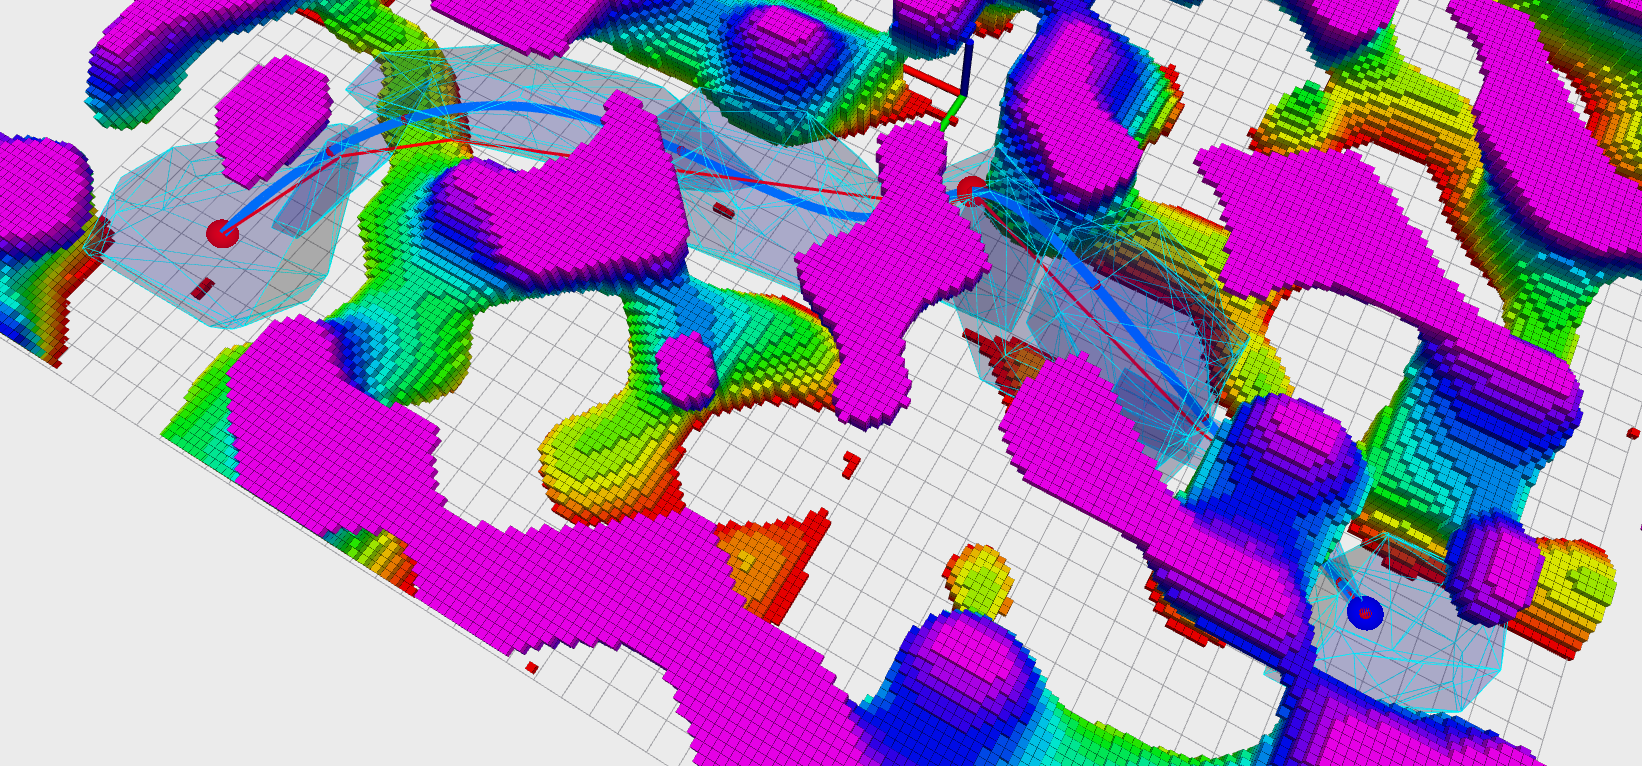
\includegraphics[width=16cm, height=7cm]{image/1.png}
        \caption{航点硬约束的全局路径轨迹效果图}\label{image1}
    \end{figure}\\
(3)\textbf{还未实现功能}


\textbf{钻运动的圈的功能、及多拓扑规划的功能暂未实现}。一方面仿真环境有限,该仿真环境是生成的静态体素地图。
第二,是该仿真是基于全局路径规划的框架,未涉及局部路径规划。\\
(4)\textbf{后续实现方向}


在EGO-PLANNER-V2既存在全局路径规划,又含有局部的路径规划。
不包含动态障碍物但仿真环境更贴近实机,其相比于EGO-PLANNER采用MINCO轨迹,方便代码修改。


尝试对EGO-PLANNER-V2进行修改,并给出一些固定航点接口等。但EGO-PLANNER-V2代码体量大、耦合程度高,存在一定难度。


\newpage
\section{2024年10月30日}
\begin{tcolorbox}[cyan]
    \begin{description}
        \item[\large \textbf{任务}]
        \item[1、] 将GCOPTER-MINCOS代码移植至EGO-PLANNER-V2
        \item[2、] 继续复现Polynomial-based 其余部分(动态环、拓扑路径规划)
    \end{description}
\end{tcolorbox}
\subsection{将GCOPTER-MINCOS代码移植至EGO-PLANNER-V2}
(1)\textbf{设计状态机FSM}


在原有状态机的基础上增加
\textbf{环的距离检测}和\textbf{固定航点重规划}。

具体逻辑:在检测到到达环(航点)附近时,规划到下一个航点的全局轨迹;
获得下一段全局轨迹之后,获得该段轨迹的局部路径规划目标点,最后进行固定航点重规划。
在飞行至环中心时,切换至原有重规划。
\begin{algorithm}[htbp]  
    \caption{\ 固定航点重规划}  
    \label{fsm}  
    \begin{algorithmic}[1]   
      \Require  无人机位置$odom\_pos\_$, 圆环中心位置$circle\_pos\_$, 固定航点重规划标志$touch\_circle\_$,当前时间$time\_now\_$,重规划界限$planning\_horizen\_$,全局规划界限$no\_replan\_thresh\_$,当前目标点$goal$
    %   \Ensure  
    \State \CASE{$ EXEC\_TRAJ $}
    \If{ $touch\_circle\_  \ \ \mathbf{and}\ \  (time\_now\_ > circle\_cross\_time\_ - 0.1\ \  \mathbf{or}\ \  (odom\_pos\_ - circle\_pos\_).norm() < 0.09)$}
            \State $cir\_ps\_.erase(cir\_ps\_.begin())$
            \State $touch\_circle\_ = false$
            \State $already\_cross = true$
            \State $have\_planed\_next\_waypoint = false$
        \EndIf
        \If{ $(goal - odom\_pos\_).norm() < no\_replan\_thresh\_\ \ \mathbf{and}\ \ planNextWaypoint()$}
            \State $have\_planed\_next\_waypoint = true$
            \If{ $!cir\_ps\_.empty()\ \ \mathbf{and}\ \ (odom\_pos\_ - circle\_pos\_).norm() < planning\_horizen\_$}
            \State $touch\_circle\_ = true$
            \State $planFromLocalTraj(1)$
            \EndIf
        \EndIf
    \end{algorithmic}  
  \end{algorithm}


(2)\textbf{定义MINCOS类}


(3)\textbf{增加固定航点重规划算法}


(4)\textbf{运行效果}


正常运行效果,如图\ref{image2}。
\begin{figure}[htbp]
    \centering
    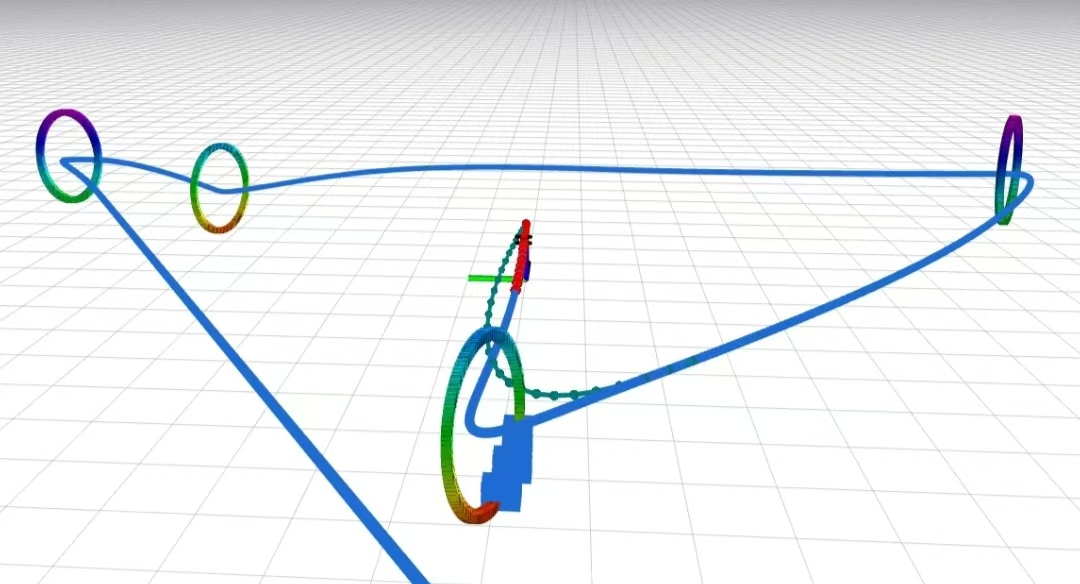
\includegraphics[width=16cm, height=7cm]{image/2.jpg}
    \caption{航点硬约束的局部路径规划全局效果图}\label{image2}
\end{figure}\\


有小概率优化之后的轨迹会打圈,并且很难从环的另一端钻出,如图\ref{image3},初步分析可能原因:


一方面是逻辑还需修改,因为固定经过环的中心即可,在需要大幅转弯时,可能存在掉头飞行的情况。


另一方面可能是优化的代价函数需修改,所采用的优化代价函数的每一项代价是采用EGO-V2的代价函数进行计算的,可能并不适用于固定航点优化。


\begin{figure}[htbp]
    \centering
    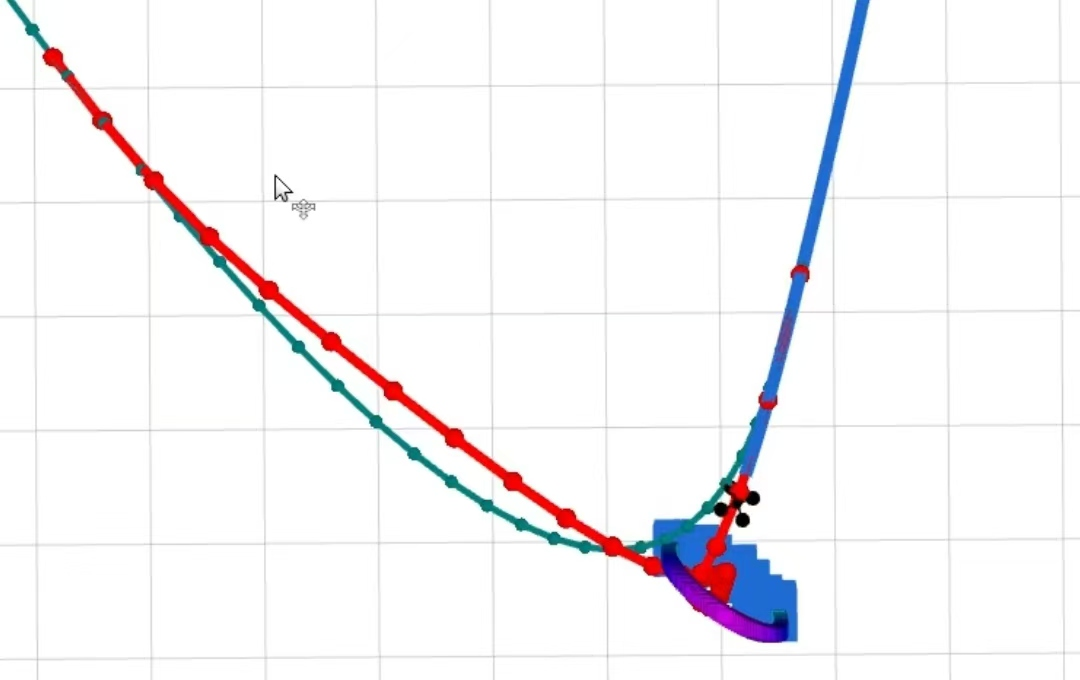
\includegraphics[width=14cm, height=8cm]{image/3.jpg}
    \caption{航点硬约束的局部路径规划失败图}\label{image3}
\end{figure}
\subsection{Time-Optimal Gate-Traversing Planner for Autonomous Drone Racing(ICRA2024)}
Code: https://github.com/FSC-Lab/TOGT-Planner
\subsubsection{论文所解决的问题}
根据所提供的门的信息,不考虑环境中的其他环境信息,计算出一条穿过所有门的时间最优且符合无人机动力学的全局轨迹。
\subsubsection{论文算法}
(1)\textbf{四旋翼无人机模型}


状态变量:$\mathbf{x} = [\mathbf{p}^W,\mathbf{q}_{WB},\mathbf{v}^W,\boldsymbol{\omega}^B]^T\in\mathbb{R}^n,n=13$,分别为世界坐标系下的位置、由机体坐标系到世界坐标系的单位四元数旋转矩阵、世界坐标系下的速度、机体坐标系下的角速度\\


输入变量:$\mathbf{u}=[f_1,f_2,f_3,f_4]^T\in \mathbb{R}^m,m=4$,依次为四个电机的推力
\begin{align}
    \dot{\mathbf{p}}  =\mathbf{v},&\quad\dot{\mathbf{q}}=\frac12\boldsymbol{\Lambda}(\mathbf{q})\left[\begin{array}{c}0\\ \boldsymbol{\omega}\end{array}\right],\\ 
    \dot{\mathbf{v}}  =\mathbf{g}+\frac1m\mathbf{R}(\mathbf{q})\mathbf{F}_{T},&\quad\dot{\boldsymbol{\omega}}=\mathbf{J}^{-1}(\boldsymbol{\tau}-\boldsymbol{\omega}\times\mathbf{J}\boldsymbol{\omega})
\end{align}
其中 
\begin{equation}
    \mathbf{F}_{T}  =\left[\begin{array}{c}0\\ 0\\ \sum f_{i}\end{array}\right],\boldsymbol{\tau}=\left[\begin{array}{c}l(f_1+f_2-f_3-f_4)\\ l(-f_1+f_2+f_3-f_4)\\ c_{\tau}(f_1-f_2+f_3-f_4)\end{array}\right].
\end{equation}
(2)\textbf{门约束的定义}\\
\textbf{球形门}:指在飞行过程中必须要经过的航点。
\begin{equation}
    \mathcal{G}_{\mathcal{B}}=\{\mathbf{p}\in\mathbb{R}^3|\|\mathbf{p}-\mathbf{p}_w\|_2\leq\delta\},
\end{equation}
其中,$\mathbf{p}_w$是球形门的中心,$\delta$是其半径。\\
\textbf{凸多边形门}:指在飞行过程中要钻过的门或隧道。
\begin{equation}
    \mathcal{G}_{\mathcal{P}}=\{\mathbf{p}\in\mathbb{R}^3|\mathbf{A}\mathbf{p}\leq\mathbf{b}\},
\end{equation}
(3)\textbf{时间最优门遍历问题}
\begin{align}
\min_{\mathbf{x},\mathbf{u},t_f}& t_{f} \\
\mathrm{s.t.}& \mathbf{x}(0)=\bar{\mathbf{x}}_0, \mathbf{x}(t_f)=\bar{\mathbf{x}}_f, \\
&\dot{\mathbf{x}}=\mathbf{f}(\mathbf{x},\mathbf{u}), \mathbf{h}(\mathbf{x},\mathbf{u})\leq0, \\
&\exists 0<t_{1}<t_{2}<...<t_{L}<t_{f}, \\
&\mathbf{h}_{\mathcal{G}^{i}}(\mathbf{p}_{\mathbf{x}(t_{i})})\leq0, 1\leq i\leq L,
\end{align}
(4)\textbf{问题转化与求解}\\
\textbf{门约束与时间解耦}
\begin{equation}
    \begin{aligned}\min_{\mathbf{P},\mathbf{T}}&T_{\Sigma}+I_{\mathcal{T}(\mathbf{P})}(\mathbf{T})\\\mathrm{s.t.}&\mathbf{h}_{\mathcal{G}^{i}}(\mathbf{p}_{i})\leq\mathbf{0}, 1\leq i\leq L,\end{aligned}
\end{equation}
其中,
\begin{equation}
    I_{\mathcal{T}(\mathbf{P})}(\mathbf{T})=\left\{\begin{array}{ll}0&,\mathrm{if~}\mathbf{T}\in\mathcal{T}(\mathbf{P})\\
        \infty&,\mathrm{if~}\mathbf{T}\notin\mathcal{T}(\mathbf{P})\end{array}\right.
\end{equation}
\begin{equation}
    \begin{aligned}\label{TP}
\mathcal{T}(\mathbf{P})=\{\mathbf{T}\in\mathbb{R}_{>}^{L+1}& \mid\exists\mathbf{x},\mathbf{u}:[0,T_\Sigma]\to\mathbb{R}^n,\mathbb{R}^m \\
\text{s.t.}& \mathbf{x}(0)=\bar{\mathbf{x}}_{0}, \mathbf{x}(T_{\Sigma})=\bar{\mathbf{x}}_{f} \\
&\dot{\mathbf{x}}=\mathbf{f}(\mathbf{x},\mathbf{u}),\mathbf{h}(\mathbf{x},\mathbf{u})\leq0 \\
&\mathbf{p}_{\mathbf{x}(t_{\Sigma_{i}})}=\mathbf{p}_{i}, 1\leq i\leq L\}.
\end{aligned}
\end{equation}
给定门的位置向量后,可行时间分配向量的集合如式\ref{TP}所示。采用MINCO轨迹能够消除尽可能多的约束,并且具有最少数量的系数,大大降低了问题的复杂性。
通过结合微分平坦特性消除对系统动力学、初始状态和终端状态的约束,而且可以确保精确的航路点遍历,从\ref{TP}中删除大量约束,只留下状态输入约束。
连续状态输入约束通过采样来定义惩罚泛函。
\begin{equation}
    \begin{aligned}
&I_{\hat{\mathcal{T}}(\mathbf{P})}(\mathbf{T})=\int_{0}^{T_{\Sigma}}\mathrm{max}[\mathbf{h}_{\Psi}(\mathbf{y}^{[s]}(t)),\mathbf{0}]^{3}dt, \\
&\approx\sum_{i=1}^{L+1}\sum_{j=0}^{\kappa_i}\max[\mathbf{h}_\Psi(\mathbf{y}^{[s]}(t_{i-1}+j\Delta t_i)),\mathbf{0}]^3\Delta t_i,
\end{aligned}
\end{equation}
(5)\textbf{门约束和时间约束}


通过将门约束和时间约束的可行解空间映射至n维欧式空间后,进行无约束优化。\\
(6)\textbf{无约束优化}
\begin{equation}
    \min_{\mathbf{D},\mathbf{K}}\quad T_{\Sigma}(\mathbf{K})+I_{\hat{\mathcal{T}}(\mathbf{P}(\mathbf{D}))}(\mathbf{T}(\mathbf{K})).
\end{equation}
推导上述函数梯度,并采用L-BFGS算法进行优化,优化完成后可由$\mathbf{D、K}$获得航点向量$\mathbf{P}$和时间向量$\mathbf{T}$,然后构建MINCO轨迹,之后通过微分平坦便可得到全状态变量和输入变量。
\subsubsection{论文启发}
本篇论文通过对穿过所有门的全局路径规划问题进行问题建模,并且采用MINCO轨迹来进行轨迹表示,
一方面能够减少优化问题中的约束,另一方面可以减少优化参数;对连续性状态输入约束采用离散化的惩罚泛函;对凸的门约束和时间约束映射至n维欧氏空间进行优化。
从本篇论文中能够了解MINCO轨迹以及几何优化方法的应用。

\newpage
\section{2024年11月12日}
\begin{tcolorbox}[cyan]
    \begin{description}
        \item[\large \textbf{任务}]
        \item[1、] 读文献学习代价函数构建方法
        \item[2、] 解决优化轨迹“打圈”的问题
        \item[3、] 文献进展报告为四部分:(1)论文所解决的问题(2)算法(3)结果(4)论文启发 
    \end{description}
\end{tcolorbox}
\subsection{Minimum Snap Trajectory Generation and Control for Quadrotors(ICRA2011)}
\subsubsection{论文所解决的问题}
论文提出了四旋翼无人机在严格约束(轨迹总时间以及航点约束)的三维空间中的控制器设计和轨迹生成方法。
论文对无人机的微分平坦特性进行了详细推导;构建minimum snap优化问题,将优化变量的解耦关系,将问题分解成四个优化问题,并转换成无量纲优化问题。
并提出飞行走廊约束方法,本文中用于无人机钻环。
\subsubsection{论文算法}
(1)\textbf{无人机微分平坦特性}


无人机动力学模型如下:
\begin{subequations}
    \begin{numcases}{}
      m\ddot{\mathbf{r}}=-mg\mathbf{z}_W+u_1\mathbf{z}_B \label{dynamic1}\\
      \dot{\boldsymbol{\omega}}_{BW}=\mathcal{I}^{-1}\left[-\boldsymbol{\omega}_{BW}\times \mathcal{I}\boldsymbol{\omega}_{BW}+\left[\begin{array}{c}u_2\\u_3\\u_4\end{array}\right]\right]\label{dynamic2}
    \end{numcases}
\end{subequations}


平坦输出:$\sigma(t) = \left[x,y,z,\psi \right]^T $。由式\ref{dynamic1}可知,机体坐标系的$Z_B$轴方向$\mathbf{z_B}$满足下式
\begin{equation}\label{zBandt}
    \mathbf{z_B}=\frac{\mathbf{t}}{\left\lVert\mathbf{t} \right\rVert },\mathbf{t}= \left[\ddot{\sigma}_1,\ddot{\sigma}_2,\ddot{\sigma}_3 +g  \right]^T
\end{equation}
给定$\psi$,可以计算出$\mathbf{x}_C = \left[\cos\sigma_4,\sin\sigma_4,0  \right]^T$,由于采用$Z-X-Y$的旋转顺序,
坐标轴\(\mathbf{x}_C\)和\(\mathbf{x}_B\)、\(\mathbf{z}_B\)在一个平面,$\mathbf{y}_B$与$\mathbf{z}_B$和$\mathbf{x}_C$正交。
因此,有
\begin{equation}\label{flatness1}
    \mathbf{y}_B=\frac{\mathbf{z}_B\times\mathbf{x}_C}{\|\mathbf{z}_B\times\mathbf{x}_C\|},\begin{array}{c}\mathbf{x}_B=\mathbf{y}_B\times\mathbf{z}_B\end{array}
\end{equation}
之后可以唯一确定从机体坐标系到世界坐标系的旋转矩阵\(^WR_B=\left[\mathbf{x}_B\ \ \mathbf{y}_B\ \ \mathbf{z}_B\right]\),
通过旋转矩阵可以确定无人机的滚动角\(\phi \)和俯仰角$\theta$。对式\ref{dynamic1}求导得
\begin{equation}\label{equ-3-14}
    m\dot{\mathbf{a}}=\dot{u}_1\mathbf{z}_B+\boldsymbol{\omega}_{BW}\times u_1\mathbf{z}_B
\end{equation}
沿\(\mathbf{z}_B\)投影可得\(\dot{u}_1=\mathbf{z}_B\cdot m\dot{\mathbf{a}} \),
并定义向量\(\mathbf{h}_\omega=\boldsymbol{\omega}_{BW}\times\mathbf{z}_B=\frac m{u_1}(\dot{\mathbf{a}}-(\mathbf{z}_B\cdot\dot{\mathbf{a}})\mathbf{z}_B)\)
为\(\frac m{u_1}\dot{\mathbf{a}}\)在\(X_B-Y_B\)平面上的投影。因此
\begin{equation}
   p=-\mathbf{h}_\omega\cdot\mathbf{y}_B,q=\mathbf{h}_\omega\cdot\mathbf{x}_B\label{equ-3-15}
\end{equation}
另外,\(r\)是\(\boldsymbol{\omega}_{BW}\)在\(\mathbf{z}_B\)方向的分量,
并将\(\boldsymbol{\omega}_{BW}\)分解为\(\boldsymbol{\omega}_{BC}+\boldsymbol{\omega}_{CW}\)能够得出
\begin{equation}\label{equ-3-16}
    r=(\omega_{BC}+\omega_{CW})\cdot\mathbf{z}_B=\omega_{CW}\cdot\mathbf{z}_B=\dot{\psi}\mathbf{z}_W\cdot\mathbf{z}_B
\end{equation}
同样,对式\ref{dynamic1}求二阶导可以得出,角加速度也可以被平坦输出及其有限阶导数的函数表示。

对于控制输入\(u\),由式\ref{dynamic1}、\ref{zBandt}可知,净推力\(u_1=m\|\mathbf{t}\|\);
另外,由于角速度和角加速度是\(z\)及其导数的函数,因此可以通过式\ref{dynamic2}来计算输入\(u_2\),\(u_3\)和\(u_4\)。
综上,四旋翼无人机系统的12个状态和4个控制输入都可以写成平坦输出\(\sigma\)及其导数的形式。

(2)\textbf{轨迹生成}


轨迹表示为$m$段$n$阶多项式轨迹,如下
\begin{equation}
    \sigma_T(t)=\left\{\begin{array}{cc}\sum_{i=0}^n\sigma_{Ti1}t^i&t_0\leq t<t_1\\\sum_{i=0}^n\sigma_{Ti2}t^i&t_1\leq t<t_2\\\vdots\\\sum_{i=0}^n\sigma_{Tim}t^i&t_{m-1}\leq t\leq t_m\end{array}\right.
\end{equation}


优化问题的构建:
代价函数包含位置$\mathbf{r_T}$的$k_r$阶导的平方和偏航角$\psi$的$k_\psi$阶导的平方,如下
\begin{equation}
    \begin{aligned}\label{costfun}
        &\min&\int_{t_0}^{t_m}\mu_r\left|\left|\frac{d^{k_r}\mathbf{r_T}}{dt^{k_r}}\right|\right|^2+\mu_\psi\frac{d^{k_\psi}\cdot\psi_\mathbf{T}}{dt^{k_\psi}}^2dt&\\
        &\text{s.t.}&\sigma_T(t_i)=\sigma_i,&i=0,...,m\\
        & &\frac{d^px_T}{dt^p}|_{t=t_j}=0\text{ or free},&j=0,m; p=1,...,k_r\\
        & &\frac{d^py_T}{dt^p}|_{t=t_j}=0\text{ or free},&j=0,m; p=1,...,k_r\\
        & &\frac{d^pz_T}{dt^p}|_{t=t_j}=0\text{ or free},&j=0,m; p=1,...,k_r\\
        & &\frac{d^p\psi_T}{dt^p}|_{t=t_j}=0\text{ or free},&j=0,m; p=1,...,k_\psi
    \end{aligned}
\end{equation}
其中,$\mu_r$、$\mu_\psi$的作用是使积分量无量纲。由于$u_2,u_3$由位置的四阶导表示,并且$u_4$由偏航角的二阶导表示,因此取$k_r=4,k_\psi=2$
将优化变量$\sigma_{Tij}=[x_{Tij},y_{Tij},z_{T\boldsymbol{i}j},\psi_{Tij}]^T$
写成$4mn\times 1$的向量$\mathbf{c}$,则问题转换为一个QP问题,如下
\begin{equation}\label{qp}
    \begin{array}{cc}\min&c^THc+f^Tc\\\mathrm{s.t.}&Ac\leq b\end{array}
\end{equation}
(3)\textbf{无量纲优化}


式\ref{costfun}中的变量$x_T,y_T,z_T,\psi_T$是解耦的,因此可以将问题分离为四个优化问题。
考虑单一无量纲变量$\tilde{\omega}(\tau)$的优化问题,如式\ref{costfun1}所示。其中$\tau$代表无量纲时间。
\begin{equation}
    \begin{aligned}\label{costfun1}
    \text{min}&\quad\quad\int_0^1\frac{d^k\tilde{w}(\tau)}{d\tau^k}^2d\tau\\
    \text{s.t.}&\quad\quad\tilde{w}(\tau_i)=\tilde{w}_i,&i=0,...,m\\
    \quad&\frac{d^p\tilde{w}(\tau)}{d\tau^p}|_{\tau=\tau_j}=0\text{ or free},&\tau_j=0,1; p=1,...,k
\end{aligned}
\end{equation}
引入时间维度$t=\alpha \tau$和变量$\omega$,定义为$w(t)=w(\alpha\tau)=\beta_1+\beta_2\tilde{w}(\tau)$。
则问题\ref{costfun1}可变换为如下问题
\begin{equation}
\begin{aligned}\label{costfun2}
    &\text{min}&&\frac{\alpha^{2k-1}}{\beta_{2}}\int_{0}^{\alpha}\frac{d^{k}w(t)}{dt^{k}}dt&&\\
    &\text{s.t.}&&w(t_{i})=\beta_{1}+\beta_{2}\tilde{w}_{i},\quad i=1,...,m\\
    &&&\frac{d^{p}w(t)}{dt^{p}}|_{t=t_{j}}=0\mathrm{~or~free},\quad t_{j}=0,\alpha; p=1,...,k
\end{aligned}
\end{equation}
在问题\ref{costfun2}中边界条件在空间维度平移了$\beta_1$缩放了$\beta_2$,在时间维度缩放了$\alpha$。
因此,如果无量纲优化问题\ref{costfun1}的最优解是$\tilde{\omega}^*$,则问题\ref{costfun2}的最优解为
\begin{equation}
    w^*(t)=\beta_1+\beta_2\tilde{w}^*\left(t/\alpha\right)
\end{equation}
\textbf{整体优化思路}:对于问题\ref{costfun},在解耦后分别与问题\ref{costfun2}对应,得到时间放缩尺度$\alpha$与
和每个变量在空间中的变换$\beta_1,\beta_2$的比例关系。每个变量的时间放缩尺度相同,空间放缩尺度可以不同。


1)时间放缩
\begin{equation}
    \mathbf{r}_T^*(t)=\mathbf{\tilde{r}}_T^*(t/\alpha), \psi_T^*(t)=\tilde{\psi}_T^*(t/\alpha).
\end{equation}


2)空间放缩
\begin{equation}
    x_T^*(t)=x_0+(x_1-x_0)\tilde{x}_T^*(t/t_1),
\end{equation}
其中,$\tilde{x}_T^*(0)=0,\tilde{x}_T^*(1)=1$,且$\tilde{y}_T,\tilde{z}_T$也满足同样的关系。\\
(4)\textbf{飞行走廊}


定义$\mathbf{t}_i$为$\mathbf{r}_i$到$\mathbf{t}_{i+1}$的单位向量,则垂直距离向量定义为
\begin{equation}
    \mathbf{d}_i(t)=(\mathbf{r}_T(t)-\mathbf{r}_i)-((\mathbf{r}_T(t)-\mathbf{r}_i)\cdot\mathbf{t}_i)\mathbf{t}_i.
\end{equation}
并定义约束
\begin{equation}\|\mathbf{d}_i(t)\|_\infty\leq\delta_i\text{ while }t_i\leq t\leq t_{i+1}.\end{equation}
其中,$\left\lVert \right\rVert _\infty  $表示无穷范数。对于$n$维向量$\mathbf{x}=(x_{1},x_{2},\ldots,x_{n})$,无穷范数定义为$\|\mathbf{x}\|_\infty=\max_{1\leq i\leq n}|x_i|$。
上述约束可以通过引入$n_c$个中间点从而合并至QP问题\ref{qp}中。
\begin{equation}
    \left|\mathbf{x}_W\cdot\mathbf{d}_i\left(t_i+\frac{j}{1+n_c}(t_{i+1}-t_i)\right)\right|\leq\delta_i\text{ for }j=1,...,n_c
\end{equation}
(5)\textbf{时间优化}


在大多数情况下,飞至某个固定点时的时间并不重要,因此可以对这些时间进行优化,找到每段轨迹最优飞行时间。
构建如下优化问题。
\begin{equation}\label{optt}
    \begin{aligned}\min&f(\mathbf{T})\\\mathrm{s.t.}&\sum T_i=t_m\\&T_i\geq0\end{aligned}
\end{equation}
其中$f(\mathbf{T})$是问题\ref{costfun}的解,时间向量$\textbf{T}= [T_1,T_2,...,T_m]$。可通过梯度下降法来求解问题\ref{optt}。
$f(\mathbf{T})$对第$i$段轨迹的时间的导数如下
\begin{equation}
    \nabla_{g_i}f=\frac{f(\mathbf{T}+h\mathbf{g}_i)-f(\mathbf{T})}h
\end{equation}
其中,向量$\mathbf{g}_i$的第$i$个元素是1,其余元素都是$\frac{-1}{m-1}$。可以使得$\sum\mathbf{g}_i=0$,对轨迹飞行总时间没有影响。

\subsubsection{论文实验结果}
(1)飞行走廊、时间优化仿真实验
\begin{figure}[htbp]
    \centering
    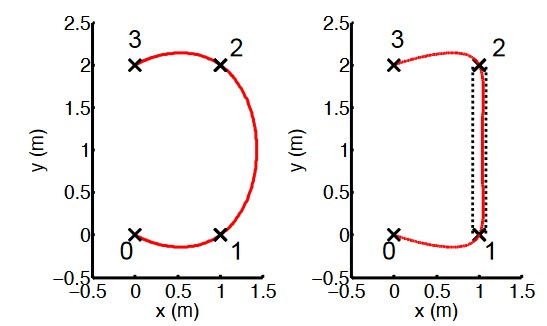
\includegraphics[width=8cm, height=4cm]{image/minimumSnap1.jpg}
    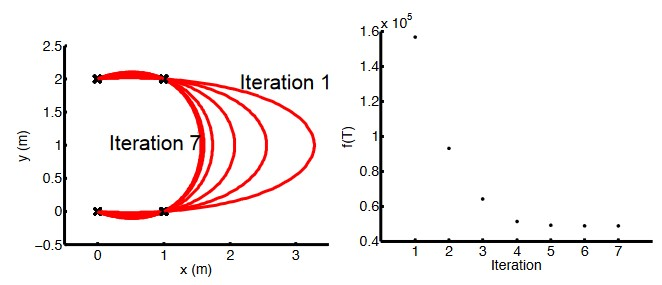
\includegraphics[width=8cm, height=4cm]{image/minimumSnap2.jpg}
    \caption{飞行走廊实验(左)  时间优化实验(右)}\label{snap1}
\end{figure}



(2)实机钻环实验
\begin{figure}[htbp]
    \centering
    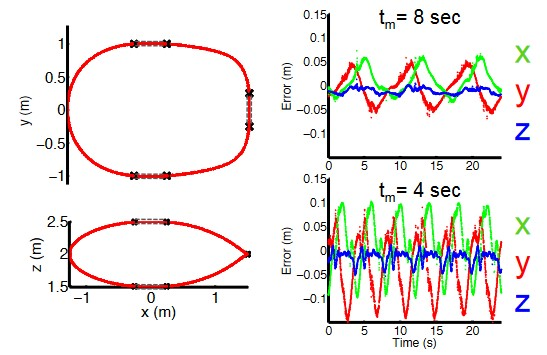
\includegraphics[width=8cm, height=5cm]{image/minimumSnap3.jpg}
    \caption{实机钻环实验}\label{snap3}
\end{figure}

\subsubsection{论文启发}(1)微分平坦


掌握无人机微分平坦特性的推导,由平坦输出获得全状态变量和全输入变量的方法。\\
(2)优化问题各维度解耦与无量纲优化


在该优化问题中优化变量是解耦的,因此优化问题可以被分解为若干个优化子问题。
并且可以将子优化问题转换为无量纲优化问题,在得到无量纲优化问题的最优解后,
通过时空放缩即可得到原问题最优解。该方法比直接求解QP问题快速,对于快速响应动态障碍物或目标非常有效\\
(3)时间重分配


总时间固定的重分配方法。\\
(4)飞行走廊思想


通过约束垂直距离向量的无穷范数,定义一个长方体形飞行走廊,并通过对轨迹采样来满足该飞行走廊约束。

\end{document}




